\documentclass[UTF8,a4paper,12pt]{ctexart}

\usepackage{booktabs}
\usepackage{caption}
\usepackage{float}
\usepackage{geometry}
\usepackage{graphicx}
\usepackage{hyperref}
\usepackage{pdflscape}
\usepackage{tabularx}
\usepackage{xurl}
\usepackage{xcolor}

\geometry{margin=2.4cm}
\hypersetup{
  colorlinks=true,
  linkcolor=blue!55!black,
  urlcolor=blue!55!black,
  citecolor=blue!55!black
}
\setlength{\parskip}{0.45em}
\setlength{\parindent}{2em}
\captionsetup{font=small,labelfont=bf}

\newcommand{\code}[1]{\texttt{\detokenize{#1}}}
\newcommand{\pathcode}[1]{\begingroup\urlstyle{tt}\nolinkurl{#1}\endgroup}
\newcommand{\cmd}[1]{{\ttfamily\footnotesize\detokenize{#1}}}
\newcolumntype{Y}{>{\raggedright\arraybackslash}X}
\newcommand{\statusok}{\textcolor{green!45!black}{ok}}
\newcommand{\statusna}{\textcolor{gray!70!black}{not applicable}}

\title{Dynesty.jl 综合测试与基准报告}
\author{Dynesty.jl migration test report}
\date{2026-06-11}

\begin{document}
\maketitle

\begin{abstract}
本报告汇总了当前 \code{Dynesty.jl} 工作树在 Julia 默认测试套件、示例脚本、parallel map backend、Python fixture 兼容性、benchmark runner、Python 脚本语法检查、formal parallel cost benchmark 审计，以及 LaTeX 编译链路上的验证结果。常规 Julia 测试通过 \code{julia --project=. -e 'using Pkg; Pkg.test()'} 全量执行并通过；formal benchmark 复用已经完成的 \code{examples/output/parallel_cost_compare} 输出，审计确认其为 \code{mode == "formal"}、18 个 run 全部 \code{ok}、9 个 \code{corner_overlay} posterior overlay plot 全部 \code{ok}，且所有 run 均使用 \code{/usr/bin/time -v} 并记录 process-tree RSS/PSS 内存字段。性能结果显示，在 cheap likelihood 下 Python multiprocessing wall time 中位数较低；在 medium/heavy likelihood 下 Julia 31 threads wall time 中位数明显低于 Python 31 worker processes。后验叠加图在 cheap、medium、heavy 三种 cost 与 3 个 repeat 上均生成成功，视觉上用于检查 Julia threaded 与 Python dynesty pool 的 posterior samples 是否一致到当前 benchmark 所需层面。
\end{abstract}

\tableofcontents
\newpage

\section{测试环境}

本报告基于当前工作树生成，未修改只读参考仓库 \code{../dynesty}，也未重跑 formal benchmark。formal benchmark 输出创建时间为 \code{2026-06-11T11:14:00.588}，其配置记录在 \code{examples/output/parallel_cost_compare/summary.json}。

\begin{table}[H]
\centering
\small
\begin{tabularx}{\textwidth}{p{0.26\textwidth}Y}
\toprule
项目 & 值与说明 \\
\midrule
Julia & \code{1.12.6}; \code{Threads.nthreads() == 32}; \code{BLAS.get_num_threads() == 1}。 \\
Python & \code{3.9.18}; executable: \pathcode{/home/czc/opt/miniconda3/bin/python3}。 \\
平台 & Linux x86\_64; Linux 6.1.174-1-MANJARO; AMD Ryzen 9 5950X 16-Core Processor; 32 logical threads。 \\
当前 \code{JULIA_NUM_THREADS} & 当前 shell 为 \code{32}; formal benchmark 的 Julia run 使用 \code{--threads=31}。 \\
\code{OPENBLAS_NUM_THREADS} & formal benchmark summary 记录为 \code{1}; 当前 shell 探针为 \code{1}。 \\
\code{OMP_NUM_THREADS} & formal benchmark summary 记录为 \code{1}; 当前 shell 探针为 unset。 \\
\code{MKL_NUM_THREADS} & formal benchmark summary 记录为 \code{1}; 当前 shell 探针为 \code{1}。 \\
Python dynesty source path & \pathcode{../dynesty/py}; 解析到 \pathcode{/home/czc/projects/working/dynesty/py}; 只读引用。 \\
正式 parallel benchmark & Julia 31 threads vs Python 31 multiprocessing worker processes; \code{queue_size=31}, \code{nlive=1500}, \code{dlogz=0.02}。 \\
\bottomrule
\end{tabularx}
\caption{测试与 benchmark 环境摘要。}
\end{table}

Python 参考快照来自 \pathcode{docs/source_snapshot.md}：\code{../dynesty} commit 前缀为 \code{3ec158de0d2b}，完整 commit hash 记录在 source snapshot 中；branch 为 \code{master}，快照时 \code{git status --short} 为 clean，Python dynesty 版本为 \code{2.1.2}。本报告没有对 \code{../dynesty} 执行修改、pull 或 branch switch。

\section{验证命令矩阵}

表 \ref{tab:test-matrix} 汇总本次报告生成前后执行的关键检查。耗时仅记录从测试输出或命令上下文可直接取得的信息；没有可靠墙钟秒数的短命令用 ``未单独计时'' 标注，避免伪造精确耗时。

\begin{landscape}
\begin{table}[p]
\centering
\scriptsize
\begin{tabularx}{\linewidth}{p{0.16\linewidth}p{0.34\linewidth}p{0.07\linewidth}p{0.10\linewidth}Y}
\toprule
test name & command & status & duration & notes \\
\midrule
Julia package/test suite & \cmd{julia --project=. -e 'using Pkg; Pkg.test()'} & \statusok & 未单独计时 & 默认 \pathcode{test/runtests.jl} 全量通过，包含 parallel、static/dynamic sampler、examples、Python fixtures、plotting helpers、Aqua。 \\
Examples tests & 同上 & \statusok & 17.0s & \code{Example scripts}: 35 pass。 \\
Parallel tests & 同上 & \statusok & 多个 testset & \code{Map backends}, \code{PoolUsage}, proposal/evolve queue, static/dynamic parallel backend tests 均通过。 \\
Benchmark runner include &
\begin{tabular}[t]{@{}l@{}}
\cmd{julia --project=. -e}\\
\cmd{'include("benchmark/parallel_cost_compare.jl");}\\
\cmd{println("runner ok")'}
\end{tabular}
& \statusok & 未单独计时 & 输出 \code{runner ok}。 \\
Python py\_compile &
\begin{tabular}[t]{@{}l@{}}
\cmd{python3 -m py_compile}\\
\cmd{benchmark/parallel_cost_corner.py}\\
\cmd{examples/pe_parallel_python.py}\\
\cmd{test/reference/python/generate_reference.py}
\end{tabular}
& \statusok & 未单独计时 & 无输出，exit code 0；未保留 \code{__pycache__}。 \\
Formal benchmark audit & 读取并审计 \pathcode{examples/output/parallel_cost_compare/summary.json} & \statusok & 未单独计时 & \code{mode=formal}; 18/18 run ok; 9/9 plot ok; \code{corner_overlay}; 全部使用 \code{/usr/bin/time -v}; RSS/PSS 字段存在。 \\
LaTeX compile check &
\begin{tabular}[t]{@{}l@{}}
\cmd{latexmk -xelatex}\\
\cmd{-interaction=nonstopmode -halt-on-error main.tex}
\end{tabular}
& \statusok & 见编译日志 & 本机 \code{xelatex}/\code{latexmk}/\code{ctexart} 可用，生成 \pathcode{docs/test_report/main.pdf}。 \\
Git whitespace check & \cmd{git diff --check} & \statusok & 未单独计时 & 提交前运行，确认无 whitespace error。 \\
\bottomrule
\end{tabularx}
\caption{测试与质量检查矩阵。}
\label{tab:test-matrix}
\end{table}
\end{landscape}

\section{迁移与兼容性测试概览}

当前迁移测试策略由 \pathcode{docs/testing.md}、\pathcode{docs/migration_matrix.md}、\pathcode{docs/compatibility.md} 与 \pathcode{test/reference/python/README.md} 共同描述。默认 CI 和本次 \code{Pkg.test()} 不依赖 live Python 或相邻 \code{../dynesty}，而是读取已经提交的 JSON/NPZ fixture。fixture 记录源 commit、Python/NumPy/SciPy 版本、容差和索引约定；带索引的 fixture 显式记录 Python 0-based 与 Julia 1-based 值。

\begin{itemize}
  \item Grade A 覆盖 public API 和核心数值函数，要求直接 Julia 测试，并在有意义时使用 Python fixture cross-check。
  \item Grade B 覆盖影响算法行为的 internal helper，要求直接或间接 Julia 测试；稳定输入输出场景使用 fixture。
  \item Grade C 覆盖 thin wrappers、display、plotting helpers、compatibility aliases 和 demo/doc helper，通过 caller tests、smoke tests 或迁移矩阵说明覆盖。
\end{itemize}

本次报告没有实现或替换新的 Python symbol，因此没有为了报告而修改 \pathcode{docs/migration_matrix.md}。兼容性差异也未发现新的未记录公共行为差异；既有差异包括 bang-form mutating API、1-based dimension indices、\code{copy_inputs=false} 默认行为、\code{res.blobs} 字段、Julia-native map backends 与 \code{PoolUsage}、Julia Serialization/JLD2/HDF5 persistence，以及 RecipesBase plotting 等，均已记录在 \pathcode{docs/compatibility.md}。

未运行的扩展项主要是需要显式环境变量的测试：
\begin{itemize}
  \item \code{DYNESTY_RUN_SLOW_TESTS=true}
  \item \code{DYNESTY_RUN_PLOT_TESTS=true}
  \item \code{DYNESTY_RUN_EXTENDED_TESTS=true}
  \item \code{DYNESTY_RUN_DISTRIBUTED_TESTS=true}
  \item \code{DYNESTY_RUN_JET_TESTS=true}
\end{itemize}
这些测试不属于默认 \code{Pkg.test()} 的 blocking 范围，本次报告将其标记为 not run，而不是把默认测试结果外推为扩展测试结果。

\section{Formal Benchmark 审计}

按照报告目标，formal benchmark 优先复用已有输出。本次没有重新运行 formal benchmark，因为 \pathcode{summary.json}、\pathcode{summary.csv}、\pathcode{plot_index.csv} 和 9 张 \pathcode{*julia_vs_python.png} 都存在，且审计结果足以支撑报告结论。审计结果见表 \ref{tab:audit}。

\begin{table}[H]
\centering
\small
\begin{tabular}{llll}
\toprule
check & expected & observed & status \\
\midrule
mode & formal & formal & ok \\
runs & 18 ok & 18/18 ok & ok \\
plots & 9 ok & 9/9 ok & ok \\
plot method & corner\_overlay & corner\_overlay & ok \\
/usr/bin/time -v & true & true & ok \\
RSS/PSS fields & present & true & ok \\
overlay PNG & 9 files & 9 files & ok \\
\bottomrule
\end{tabular}

\caption{formal parallel cost benchmark 输出审计。}
\label{tab:audit}
\end{table}

benchmark 配置为 \code{nlive=1500}、\code{dlogz=0.02}、\code{queue_size=31}、\code{sleep_ms=0}。Julia run 使用 31 threads 与 \code{proposal_scheduler=auto}；Python run 使用 \code{multiprocessing.Pool} 与 31 worker processes。三种 likelihood cost 的 work size 分别为 \code{cheap=0}、\code{medium=2000}、\code{heavy=10000}。所有 run 的 \code{used_usr_bin_time} 均为 true，同时保留 \code{time_max_rss_kb}、\code{process_tree_peak_rss_kb} 和 \code{process_tree_peak_pss_kb} 等字段。

\section{Parallel Cost Benchmark 结果}

表 \ref{tab:bench-summary} 从 \code{summary.json}/\code{summary.csv} 提取 cheap、medium、heavy 三种 likelihood cost 下 Julia/Python 的 wall time、CPU utilization、RSS、PSS、nsamples、logz/logzerr。每个 cost 与 implementation 有 3 次 repeat；表中 wall time 同时给出 median 与 min--max range。

\begin{landscape}
\begin{table}[p]
\centering
\small
\resizebox{\linewidth}{!}{\input{tables/benchmark_summary.tex}}
\caption{Julia/Python formal parallel cost benchmark 汇总。CPU utilization 为 total CPU seconds / wall time；RSS/PSS 均为 process tree peak KB。}
\label{tab:bench-summary}
\end{table}
\end{landscape}

RSS 与 PSS 的口径不同。RSS（Resident Set Size）按进程统计驻留物理页，并在多进程场景中容易把共享页在多个进程上重复计数；因此 Python multiprocessing 的 process-tree RSS 往往显著偏高。PSS（Proportional Set Size）会按共享页的进程数分摊内存，更适合跨单进程多线程 Julia 与多进程 Python 的 process tree 比较。本报告在讨论内存时优先查看 PSS，同时保留 RSS 以便与常见系统工具口径对应。

从中位数看，cheap cost 下 Python wall time 为 3.82s，Julia 为 14.38s；medium cost 下 Julia 为 14.39s，Python 为 37.34s；heavy cost 下 Julia 为 14.90s，Python 为 43.50s。PSS 中位数方面，Julia 三组约为 942,168 KB、901,831 KB、922,647 KB；Python 三组约为 213,612 KB、218,819 KB、218,415 KB。RSS 中位数方面，Python 三组约为 1,602,416 KB、1,608,788 KB、1,606,440 KB，受 multiprocessing 共享页重复计数影响，不能单独作为跨执行模型内存优劣结论。

附录表 \ref{tab:bench-runs} 列出全部 18 个 run 的逐次结果，以便追踪 repeat-level 波动和 evidence 数值。

\section{Posterior Overlay Plots}

本报告从 benchmark plot 输出目录复制 9 张 \code{*julia_vs_python.png} 到 \pathcode{docs/test_report/figures/}，避免提交 \code{examples/output/}。每张图比较同一 \code{cost} 与 \code{repeat} 下 Julia threaded 与 Python dynesty pool 的 posterior samples 叠加；蓝色为 \code{Dynesty.jl} threaded，橙色为 Python dynesty pool，黑色 marker 为 true value。

\begin{figure}[H]
\centering
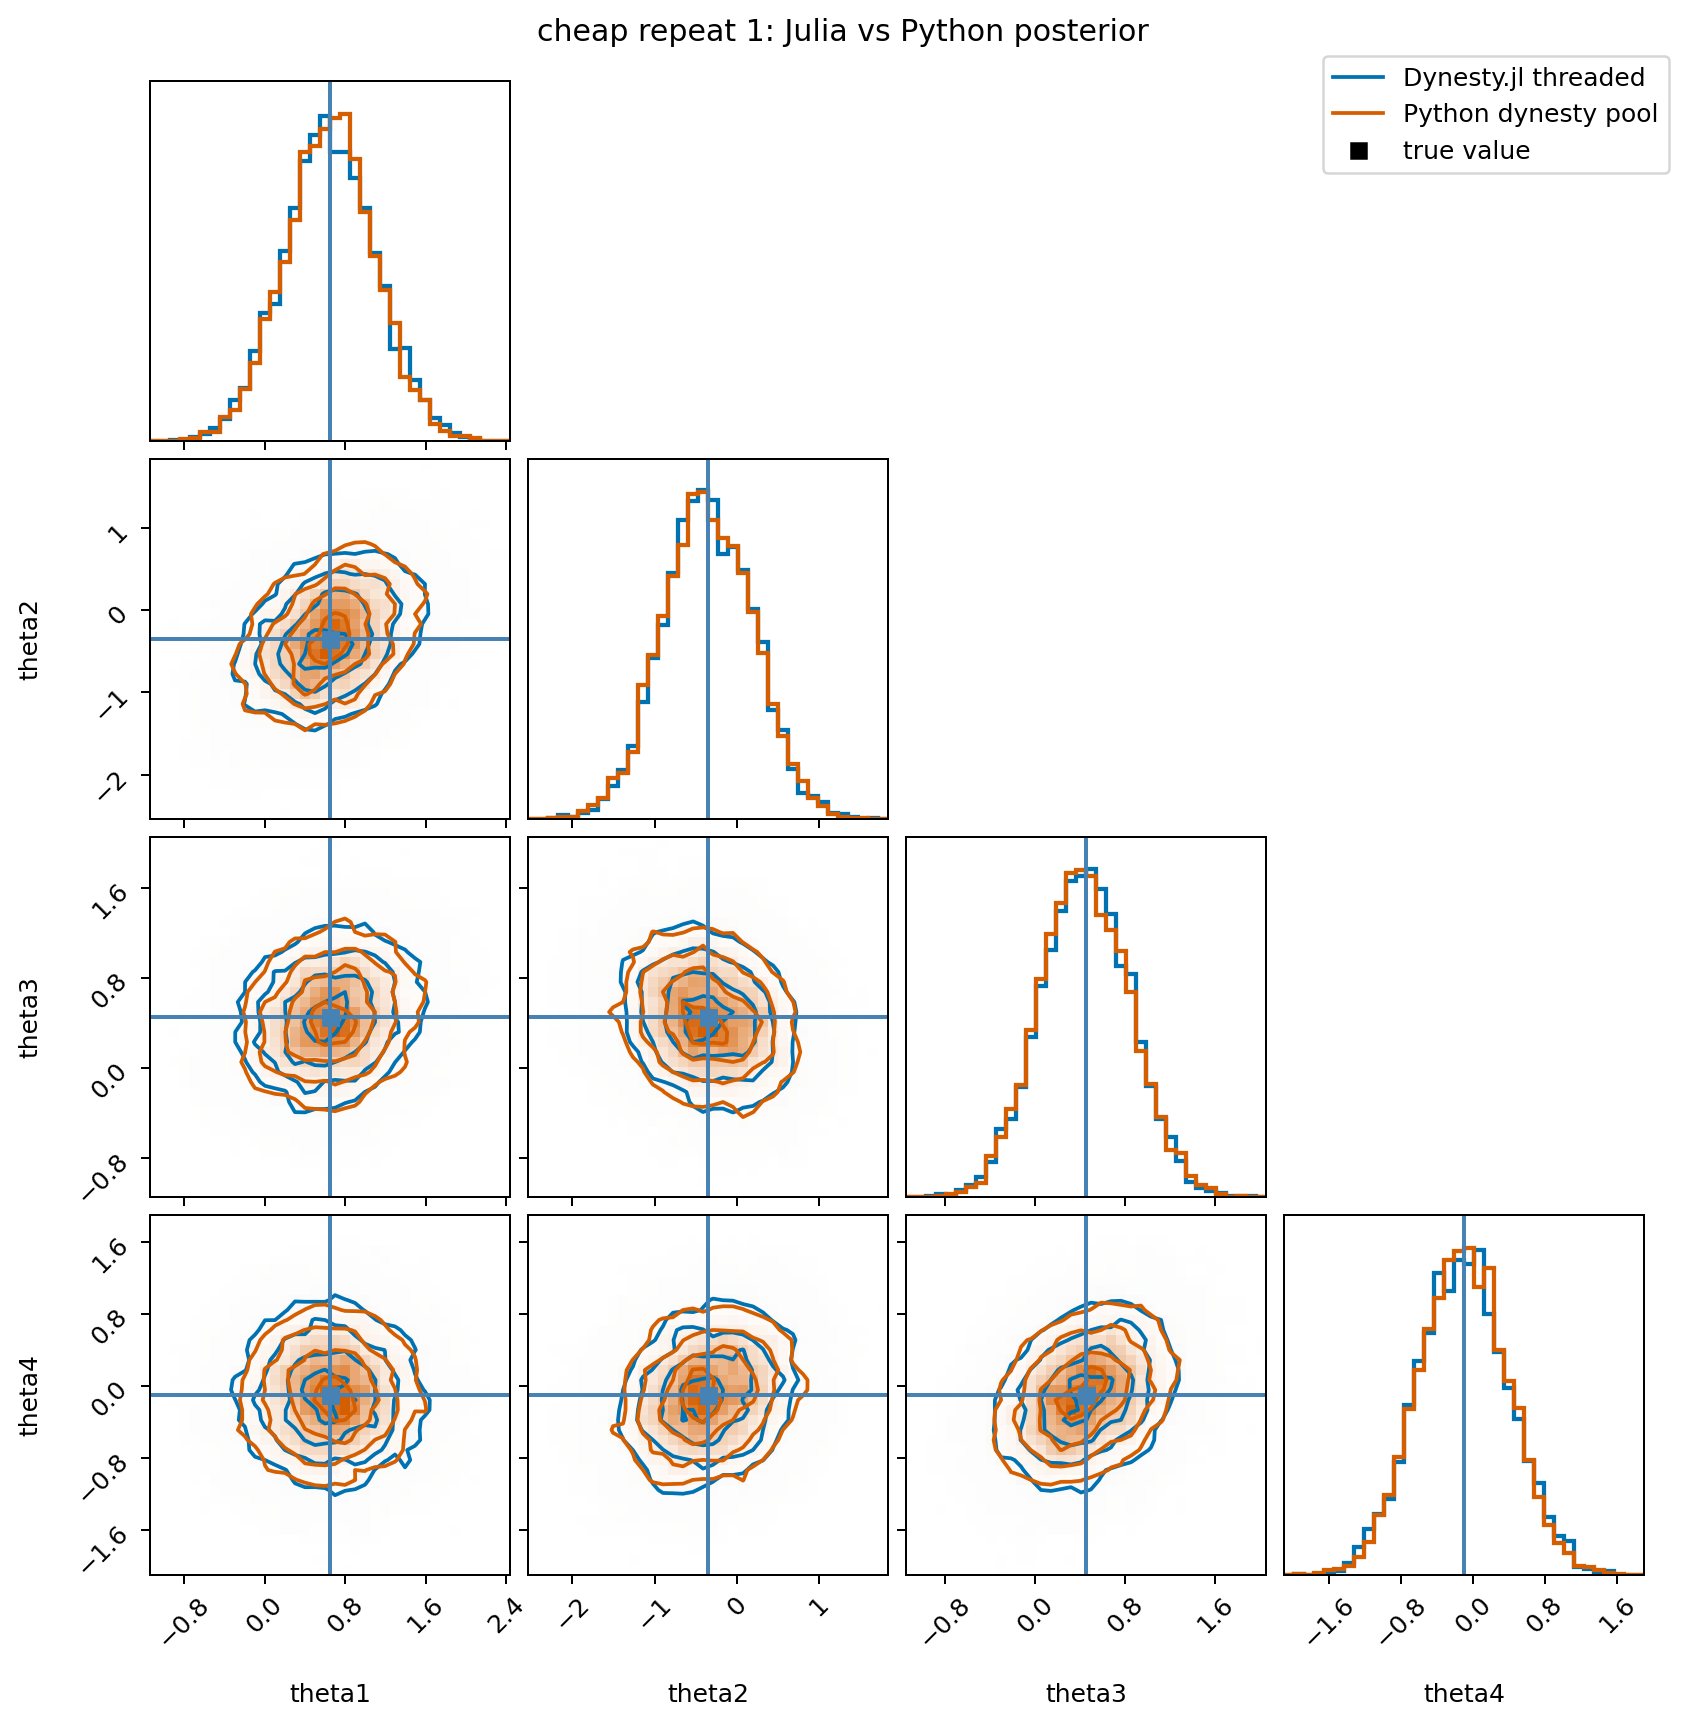
\includegraphics[width=0.90\textwidth]{figures/corner_cheap_repeat1_julia_vs_python.png}
\caption{cheap repeat 1 posterior overlay。蓝色为 Dynesty.jl threaded，橙色为 Python dynesty pool，黑色 marker 为 true value。}
\label{fig:cheap-r1}
\end{figure}

\begin{figure}[H]
\centering
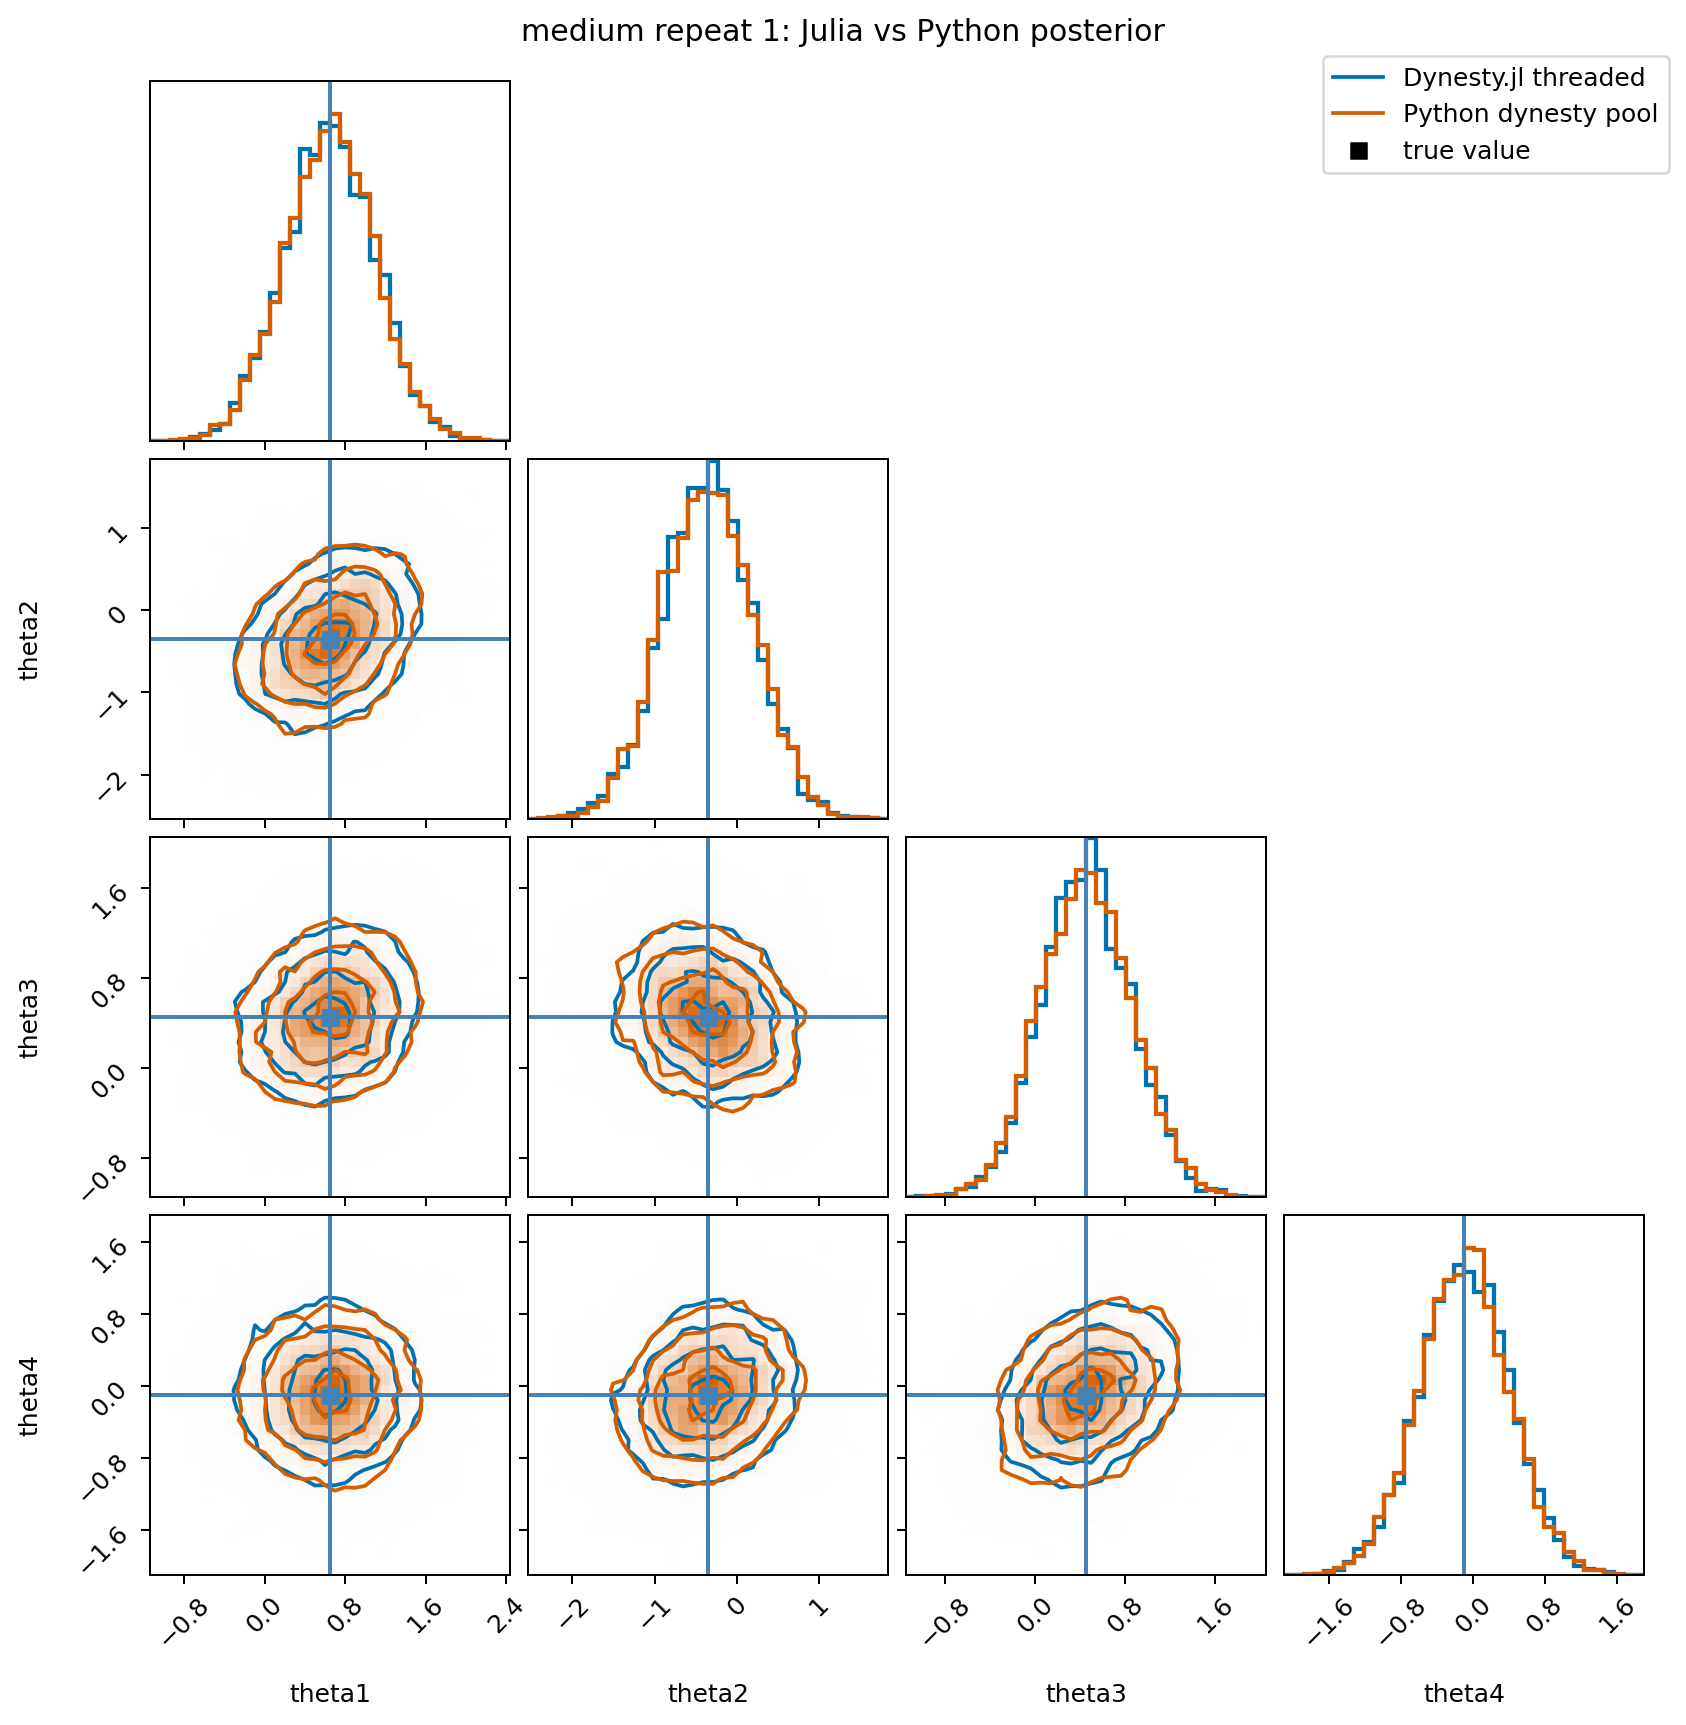
\includegraphics[width=0.90\textwidth]{figures/corner_medium_repeat1_julia_vs_python.png}
\caption{medium repeat 1 posterior overlay。蓝色为 Dynesty.jl threaded，橙色为 Python dynesty pool，黑色 marker 为 true value。}
\label{fig:medium-r1}
\end{figure}

\begin{figure}[H]
\centering
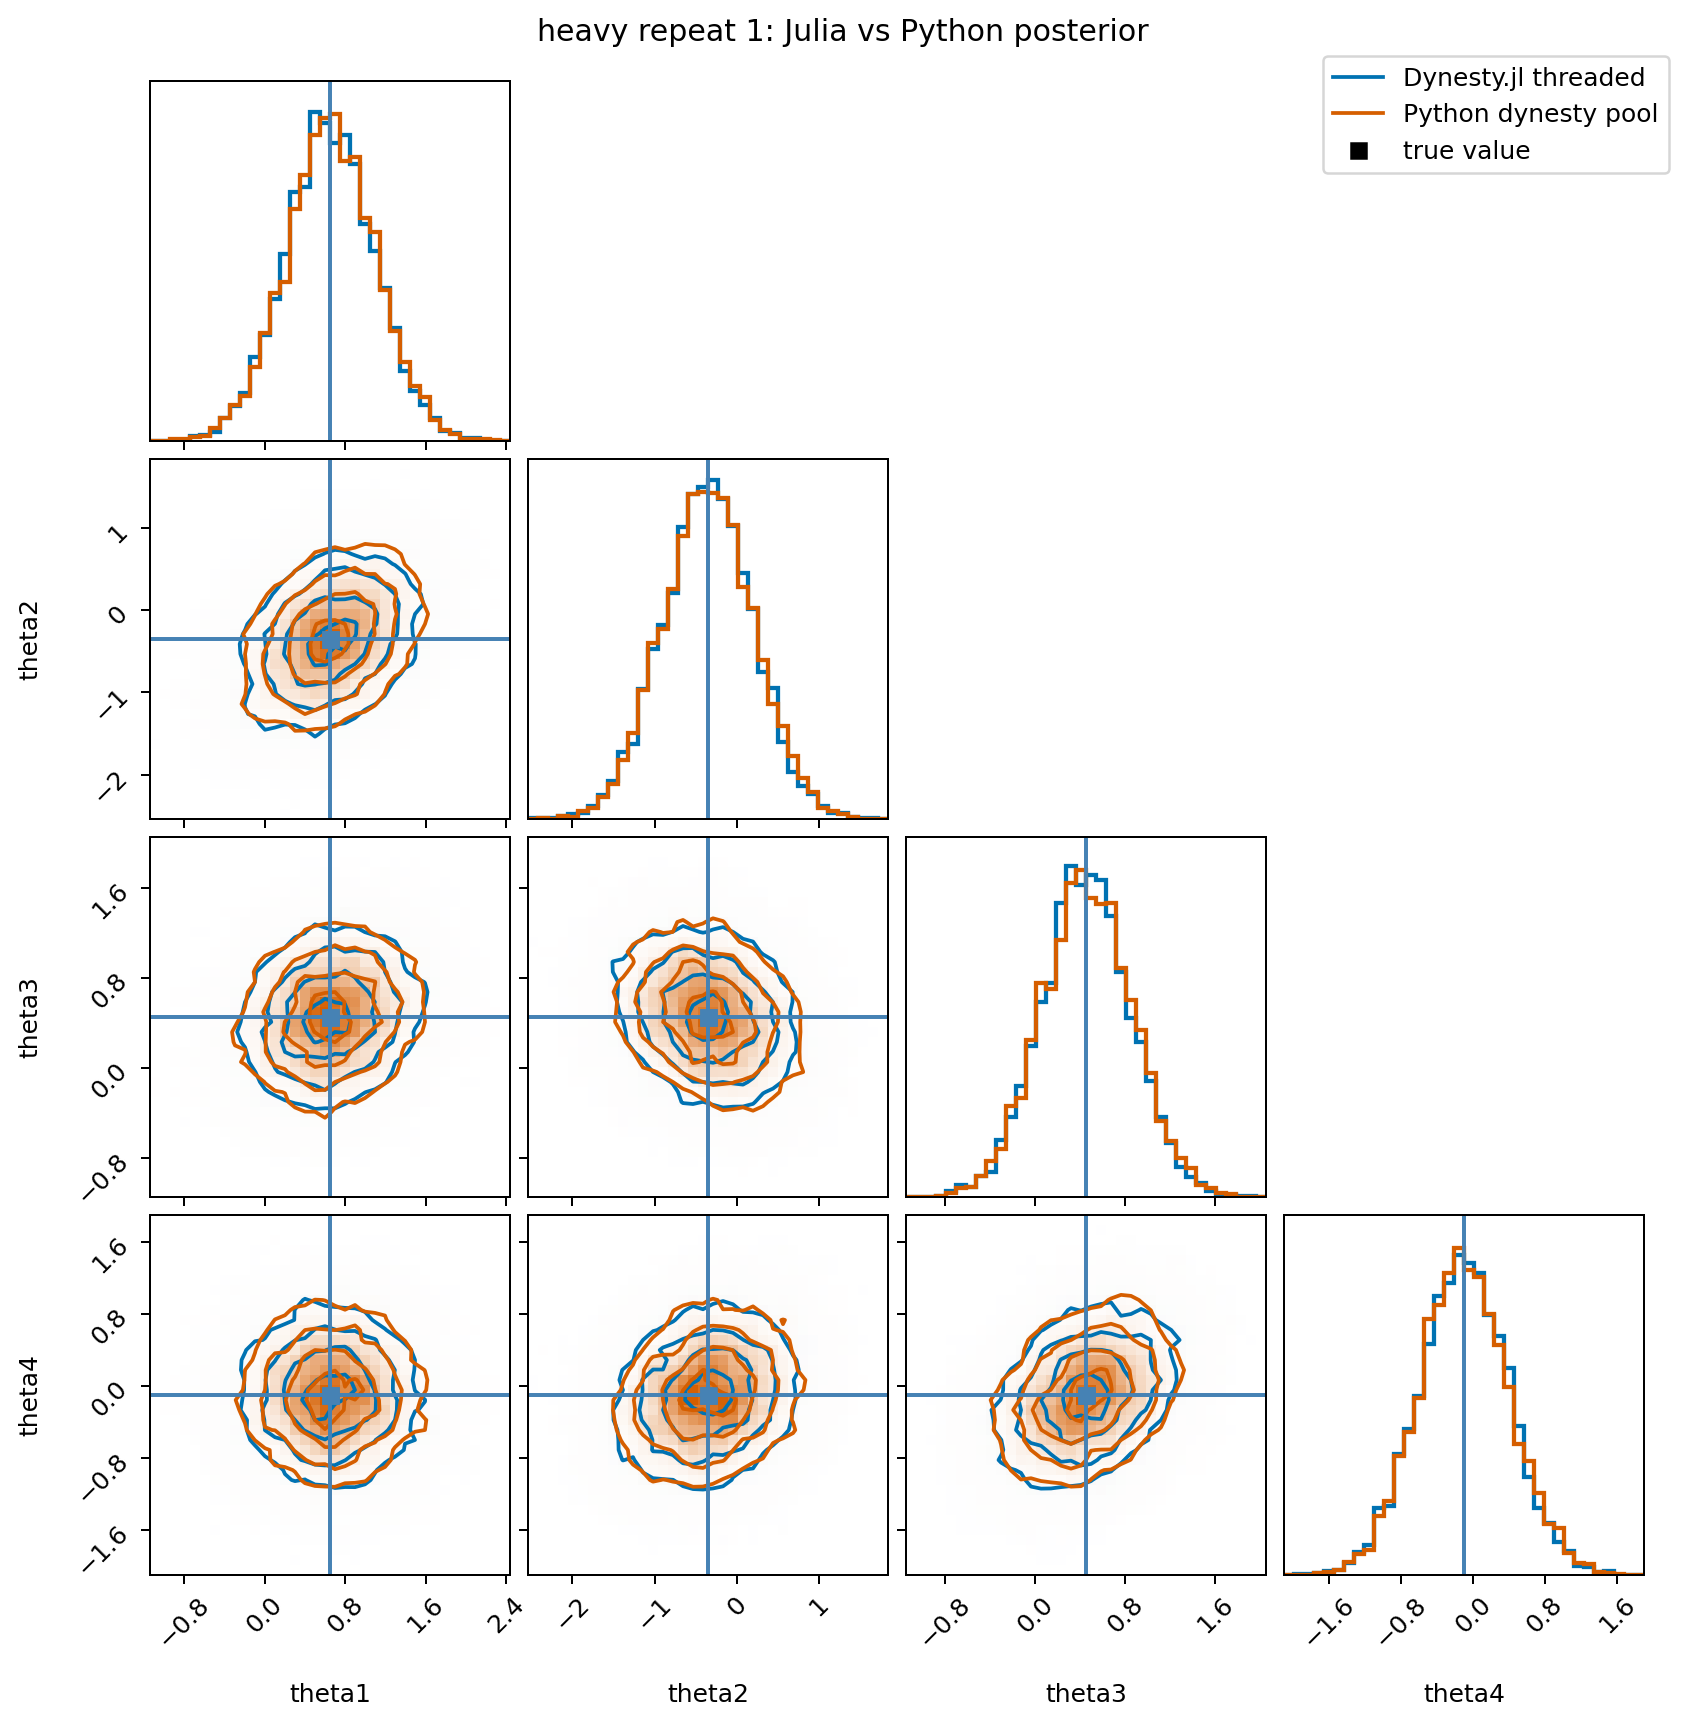
\includegraphics[width=0.90\textwidth]{figures/corner_heavy_repeat1_julia_vs_python.png}
\caption{heavy repeat 1 posterior overlay。蓝色为 Dynesty.jl threaded，橙色为 Python dynesty pool，黑色 marker 为 true value。}
\label{fig:heavy-r1}
\end{figure}

全部 9 张 overlay 图见附录表 \ref{tab:plot-index}；其文件均已复制到报告目录并纳入提交范围。

\section{结论与剩余风险}

本次常规 Julia package/test suite 全量通过，且 \code{test/runtests.jl} 覆盖了 parallel、examples、Python fixtures、plotting helpers 和 Aqua quality checks。benchmark runner include check 与 Python \code{py_compile} 也通过。formal benchmark 没有重跑，而是复用已有 \code{examples/output/parallel_cost_compare} 输出；审计确认该输出完整、一致，并且记录了 \code{/usr/bin/time -v} 与 process-tree RSS/PSS 指标。

posterior overlay 图在 cheap、medium、heavy 三种 cost 的 3 次 repeat 上全部生成成功；代表图和附录列表显示 Julia/Python 后验叠加比较已经可用于可视化层面的一致性检查。性能方面，当前 benchmark 下 Python multiprocessing 在 cheap likelihood 上 wall time 更低；当 likelihood cost 提升到 medium/heavy 后，Julia threaded 的 wall time 中位数更低。内存方面，RSS 与 PSS 结论必须分开读取：Python multiprocessing RSS 受共享页重复计数影响，PSS 更适合与 Julia threaded 的 process-tree memory 对照。

剩余风险包括：nested sampling 与 posterior visualization 受随机性和有限 repeat 数影响；性能结论依赖 AMD Ryzen 9 5950X、当前 Julia/Python/BLAS/线程设置和操作系统调度；Python multiprocessing memory accounting 的 RSS/PSS 解释依赖 Linux \code{/proc} 口径；扩展测试 flags 未在本次默认报告中打开；future benchmark 输出若更新，应重新运行 \code{docs/test_report/generate_assets.py} 并重新编译 PDF。

\appendix
\section{全部 Benchmark Run}

\begin{landscape}
\begin{table}[p]
\centering
\scriptsize
\setlength{\tabcolsep}{3pt}
\renewcommand{\arraystretch}{0.88}
\resizebox{0.96\linewidth}{!}{\begin{tabular}{lllllllllll}
\toprule
cost & impl & rep & wall s & CPU util. & RSS KB & PSS KB & nsamples & logz & logzerr & status \\
\midrule
cheap & julia & 1 & 14.38 & 3.04 & 1,027,952 & 942,168 & 17,412 & -6.68684 & 0.06032 & ok \\
cheap & julia & 2 & 14.11 & 3.00 & 1,037,576 & 951,968 & 17,365 & -6.66373 & 0.06024 & ok \\
cheap & julia & 3 & 14.47 & 3.06 & 1,022,420 & 937,667 & 17,392 & -6.67551 & 0.06041 & ok \\
cheap & python & 1 & 4.53 & 1.86 & 1,601,440 & 213,612 & 17,404 & -6.68693 & 0.06067 & ok \\
cheap & python & 2 & 3.60 & 2.32 & 1,602,416 & 215,042 & 17,566 & -6.79324 & 0.06101 & ok \\
cheap & python & 3 & 3.82 & 2.16 & 1,602,688 & 212,428 & 17,467 & -6.72226 & 0.06086 & ok \\
medium & julia & 1 & 14.39 & 3.12 & 967,948 & 883,097 & 17,389 & -6.67271 & 0.06048 & ok \\
medium & julia & 2 & 14.43 & 2.97 & 999,464 & 913,747 & 17,526 & -6.76417 & 0.06087 & ok \\
medium & julia & 3 & 14.36 & 2.90 & 986,556 & 901,831 & 17,471 & -6.73004 & 0.06076 & ok \\
medium & python & 1 & 37.26 & 9.72 & 1,608,788 & 217,776 & 17,544 & -6.77774 & 0.06097 & ok \\
medium & python & 2 & 37.34 & 9.56 & 1,611,076 & 219,379 & 17,404 & -6.68747 & 0.06063 & ok \\
medium & python & 3 & 38.08 & 9.63 & 1,601,988 & 218,819 & 17,527 & -6.76280 & 0.06078 & ok \\
heavy & julia & 1 & 14.90 & 3.42 & 1,033,952 & 948,655 & 17,502 & -6.74917 & 0.06088 & ok \\
heavy & julia & 2 & 14.86 & 3.54 & 992,624 & 906,797 & 17,444 & -6.71222 & 0.06067 & ok \\
heavy & julia & 3 & 14.93 & 3.54 & 1,007,436 & 922,647 & 17,416 & -6.69062 & 0.06064 & ok \\
heavy & python & 1 & 49.27 & 35.78 & 1,606,440 & 218,759 & 17,425 & -6.69573 & 0.06045 & ok \\
heavy & python & 2 & 43.50 & 39.93 & 1,610,588 & 216,908 & 17,391 & -6.67325 & 0.06032 & ok \\
heavy & python & 3 & 41.44 & 42.17 & 1,605,772 & 218,415 & 17,291 & -6.60632 & 0.06007 & ok \\
\bottomrule
\end{tabular}
}
\caption{18 个 formal benchmark run 的逐次结果。}
\label{tab:bench-runs}
\end{table}
\end{landscape}

\section{全部 Posterior Overlay Plot}

\begin{landscape}
\begin{table}[p]
\centering
\small
\resizebox{\linewidth}{!}{\begin{tabular}{lllllllll}
\toprule
cost & rep & file & method & status & Julia n & Python n & Julia logz & Python logz \\
\midrule
cheap & 1 & corner\_cheap\_repeat1\_julia\_vs\_python.png & corner\_overlay & ok & 17,412 & 17,404 & -6.68684 & -6.68693 \\
cheap & 2 & corner\_cheap\_repeat2\_julia\_vs\_python.png & corner\_overlay & ok & 17,365 & 17,566 & -6.66373 & -6.79324 \\
cheap & 3 & corner\_cheap\_repeat3\_julia\_vs\_python.png & corner\_overlay & ok & 17,392 & 17,467 & -6.67551 & -6.72226 \\
medium & 1 & corner\_medium\_repeat1\_julia\_vs\_python.png & corner\_overlay & ok & 17,389 & 17,544 & -6.67271 & -6.77774 \\
medium & 2 & corner\_medium\_repeat2\_julia\_vs\_python.png & corner\_overlay & ok & 17,526 & 17,404 & -6.76417 & -6.68747 \\
medium & 3 & corner\_medium\_repeat3\_julia\_vs\_python.png & corner\_overlay & ok & 17,471 & 17,527 & -6.73004 & -6.76280 \\
heavy & 1 & corner\_heavy\_repeat1\_julia\_vs\_python.png & corner\_overlay & ok & 17,502 & 17,425 & -6.74917 & -6.69573 \\
heavy & 2 & corner\_heavy\_repeat2\_julia\_vs\_python.png & corner\_overlay & ok & 17,444 & 17,391 & -6.71222 & -6.67325 \\
heavy & 3 & corner\_heavy\_repeat3\_julia\_vs\_python.png & corner\_overlay & ok & 17,416 & 17,291 & -6.69062 & -6.60632 \\
\bottomrule
\end{tabular}
}
\caption{全部 9 张 Julia-vs-Python posterior overlay plot。}
\label{tab:plot-index}
\end{table}
\end{landscape}

\end{document}
